\documentclass{beamer}
\usepackage{amsmath,amsbsy,amsopn,amstext,amsfonts,amssymb}
\usepackage{isomath}
\usepackage{ulem}
%\linespread{1.6}  % double spaces lines
\usepackage{graphicx}
\usepackage{subfigure}
\usepackage{color}
\usepackage{optidef}  % define optimization problems
\usepackage{multicol}  % multiple columns
\usepackage{listings} % for python code
\usepackage{mathrsfs}

\usepackage{polynom}
\newcommand{\adj}{\mathrm{adj}}
\newcommand{\constrainedmin}[3]{
		\begin{mini*}|s|
		{#2}{#1}{}{}
		\addConstraint{#3}
		\end{mini*}
}

\newcommand{\rwbcomment}[1]{{\color{blue}RWB:#1}}
\newcommand{\defeq}{\stackrel{\triangle}{=}}
\newcommand{\abs}[1]{\left|#1\right|}
\newcommand{\norm}[1]{\left\|#1\right\|}
\newcommand{\iprod}[1]{\left<#1\right>}
\newcommand{\ellbf}{\boldsymbol{\ell}}
\newcommand{\nubf}{\boldsymbol{\nu}}
\newcommand{\mubf}{\boldsymbol{\mu}}
\newcommand{\abf}{\mathbf{a}}
\newcommand{\bbf}{\mathbf{b}}
\newcommand{\cbf}{\mathbf{c}}
\newcommand{\dbf}{\mathbf{d}}
\newcommand{\ebf}{\mathbf{e}}
\newcommand{\fbf}{\mathbf{f}}
\newcommand{\gbf}{\mathbf{g}}
\newcommand{\hbf}{\mathbf{h}}
\newcommand{\ibf}{\mathbf{i}}
\newcommand{\jbf}{\mathbf{j}}
\newcommand{\kbf}{\mathbf{k}}
\newcommand{\lbf}{\mathbf{l}}
\newcommand{\mbf}{\mathbf{m}}
\newcommand{\nbf}{\mathbf{n}}
\newcommand{\obf}{\mathbf{o}}
\newcommand{\pbf}{\mathbf{p}}
\newcommand{\qbf}{\mathbf{q}}
\newcommand{\rbf}{\mathbf{r}}
\newcommand{\sbf}{\mathbf{s}}
\newcommand{\tbf}{\mathbf{t}}
\newcommand{\ubf}{\mathbf{u}}
\newcommand{\vbf}{\mathbf{v}}
\newcommand{\wbf}{\mathbf{w}}
\newcommand{\xbf}{\mathbf{x}}
\newcommand{\ybf}{\mathbf{y}}
\newcommand{\zbf}{\mathbf{z}}
\newcommand{\Jbf}{\mathbf{J}}
\newcommand{\Acal}{\mathcal{A}}
\newcommand{\Bcal}{\mathcal{B}}
\newcommand{\Lcal}{\mathcal{L}}
\newcommand{\Ncal}{\mathcal{N}}
\newcommand{\Rcal}{\mathcal{R}}
\definecolor{darkolivegreen}{rgb}{0.33, 0.42, 0.18}

\makeatletter
\newenvironment<>{proofstart}[1][\proofname]{%
    \par
    \def\insertproofname{#1\@addpunct{.}}%
    \usebeamertemplate{proof begin}#2}
  {\usebeamertemplate{proof end}}
\newenvironment<>{proofcont}{%
  \setbeamertemplate{proof begin}{\begin{block}{}}
    \par
    \usebeamertemplate{proof begin}}
  {\usebeamertemplate{proof end}}
\newenvironment<>{proofend}{%
    \par
    \pushQED{\qed}
    \setbeamertemplate{proof begin}{\begin{block}{}}
    \usebeamertemplate{proof begin}}
  {\popQED\usebeamertemplate{proof end}}
\makeatother

\title{ECEn 671: Mathematics of Signals and Systems}
\author{Randal W. Beard}
\institute{Brigham Young University}
\date{\today}

\begin{document}

%-------------------------------
\begin{frame}
	\titlepage
\end{frame}


%%%%%%%%%%%%%%%%%%%%%%%%%%%%%%%%%%%%%%%%%%%%%%%%%%%%%%%%%%%%%%%%%%%%%%%
\section{Orthogonality}
\frame{\sectionpage}

%----------------------------------
\begin{frame}\frametitle{Orthogonality}
Let $x,y \in \mathbb{X}$ where $\mathbb{X}$ is an inner product space.  Then the angle between $x$ and $y$ is 
\[ 
\theta = cos^{-1}\left( \frac{\iprod{ x,y }}{\norm{ x}  \norm{ y} } \right). 
\]
i.e.
\[ 
\iprod{ x,y } = \norm{ x}  \norm{ y}  cos \theta 
\]
\end{frame}

%----------------------------------
\begin{frame}\frametitle{Orthogonality, cont.}

\begin{definition}[Colinear]
Two vectors $x,y \in \mathbb{X}$ are said to be \underline{colinear} if 
\[ 
\theta = 180*n \qquad n = 0, \pm 1, \pm 2, \ldots 
\]
\end{definition}

\begin{definition}[Orthogonal] 
Two vectors $x,y \in \mathbb{X}$ are said to be \underline{orthogonal} if 
\[ 
\theta = 90*n \qquad n = \pm 1, \pm 3, \pm 5, \ldots 
\]
i.e., $\iprod{ x,y } = 0$.
\end{definition}

\vspace{1cm}

If $\iprod{ x,y } = 0$ we write $x \perp y$.\\

\end{frame}

%----------------------------------
\begin{frame}\frametitle{Orthogonality, cont.}

\begin{example}[Vectors in $L_2[0,2\pi)$]
The functions $x=sin(t)$ and $y = cos(t)$ are orthogonal since 
\[ 
\iprod{ x,y } = \int_{0}^{2\pi}sin(t)cos(t)dt = 0.
\]
\end{example}

\begin{example}[Vectors in $\ellbf$]
The sequences 
\begin{align*}
x &= (1, 1, 1, 1, 0, 0, \dots ) \\	
y &= (1, -1, 1, -1, 1, \dots)
\end{align*}
are orthogonal since 
\[ 
\iprod{ x,y } = \sum_{i=1}^\infty x_i y_i = 0.
\]
\end{example}
\end{frame}

%----------------------------------
\begin{frame}\frametitle{Other useful inner products and norms: Weighting}
\begin{definition}[Positive Definite Matrix]
A matrix $W : \mathbb{R}^k \to \mathbb{R}^k$ is \underline{positive definite} (PD) if $\forall x \in \mathbb{R}^k \quad \quad x^TWx > 0$\\
\begin{itemize}
  \item $W$ is \underline{positive semi-definite} (PSD) if $x^TWx \geq 0$
  \item $W$ is \underline{negative definite} (ND) if $x^TWx < 0 \qquad \forall x \in \mathbb{R}^k$
  \item $W$ is \underline{negative semi-definite} (NSD) if $x^TWx \leq 0 \qquad \forall x \in \mathbb{R}^k$
  \item Otherwise it is indefinite
\end{itemize}
\end{definition}
\end{frame}

%----------------------------------
\begin{frame}\frametitle{Examples of positive definiteness}
\begin{itemize}
\item $W = \left( \begin{array}{cc} 1 & 0 \\ 0 & 1 \end{array} \right)$ is PD since
\[ x^TWx = x_1^2 + x_2^2 > 0 \qquad \forall x \in \mathbb{R}^2 \]
\item $W = \left( \begin{array}{cc} 1 & 0 \\ 0 & 0 \end{array} \right)$ is PSD since
\[ x^TWx = x_1^2 = 0 \qquad \forall x = \left( \begin{array}{c} 0\\\alpha\end{array} \right) \neq 0 \]
\item $W = \left( \begin{array}{cc} -1 & 0 \\ 0 & 1 \end{array} \right)$ is indefinite since
\[ x^TWx = -x_1^2 + x_2^2 \] which can be positive or negative depending on $x$.
\end{itemize}
\end{frame}

%----------------------------------
\begin{frame}\frametitle{Examples of Inner Products}	

\noindent{\bf Weighted Inner Products and Norms}

If $W > 0$ then $\iprod{ x,y }_W = x^HWy$ is a valid inner product which induces the weighted norm $\norm{ x }_W = (x^HWx)^{\frac{1}{2}}$ 

\noindent We can define weighted inner products for functions:
\[ 
\iprod{ f,g }_W = \int f(t) g(t) w(t) dt 
\]
where $w(t) > 0$ except on a set of measure zero.
\end{frame}

%----------------------------------
\begin{frame}\frametitle{Examples of Inner Products}	
\begin{definition}[Expectation]
Expectation is a weighted inner product with weight $f_{\mathbb{X}\mathbb{Y}}(x,y)$
\begin{flalign*}
\iprod{ \mathbb{X}, \mathbb{Y} } &= \int xyf_{\mathbb{X}\mathbb{Y}}(x,y) dx dy
&= E[\mathbb{X}\mathbb{Y}]
\end{flalign*}
if $\mathbb{X}$ is a zero mean then
\[ \iprod{ x,x} = var(x)\] is the norm induced by $E[\cdot \cdot]$
\end{definition}
\end{frame}

%----------------------------------
\begin{frame}\frametitle{Examples of Inner Products}	
\begin{itemize}
\item	Let $\mathbb{I}(m,n)$ be the set of grayscale images with $m\times n$ pixels, each valued between $[0, 255]$.  
\item A valid inner on $\mathbb{I}(m,n)$ is given by
	\[
	\iprod{I, J} = \sum_{u=1}^m \sum_{v=1}^n I(u,v)J(u,v), \qquad \forall I, J \in \mathbb{I}(m,n).
	\]
\end{itemize}

\end{frame}


%----------------------------------
\begin{frame}\frametitle{Orthogonal Subspaces}
	
\begin{definition}[Orthogonal Subspaces] Let $V,W$ be subspaces of $S$.  $V \perp W$ if 
\[\forall v \in V \text{ and  } \forall w \in W, \qquad \iprod{ v,w } = 0\]
\end{definition}
\begin{definition}[Orthogonal Complement]
$V^{\perp}$, called the orthogonal complement of $V$, is  the set
\[ V^{\perp} = \{ x \in S : \forall v \in V, \iprod{ x,v} = 0 \} \]	
\end{definition}

\end{frame}

%----------------------------------
\begin{frame}\frametitle{Orthogonal Subspaces, cont.}
\begin{example}
Let $S=\mathbb{R}^2$ and $V = \left\{ \left( \begin{array}{c} \alpha\\0\end{array}\right), \alpha \in \mathbb{R} \right\}$ 
then $V^{\perp} = \left\{ \left( \begin{array}{c} 0\\\alpha\end{array}\right), \alpha \in \mathbb{R} \right\}$

\begin{center}
 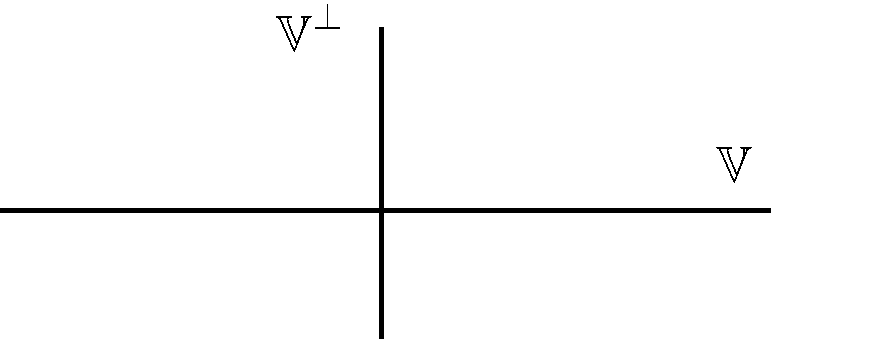
\includegraphics[width=2in]{figures/chap2_orthogonal_subspaces}		
\end{center}

\end{example}

\end{frame}

%----------------------------------
\begin{frame}\frametitle{Orthogonal Subspaces, cont.}
	
\begin{theorem}
Let $V$ and $W$ be subspaces of an inner product space $S$ (not necessarily Hilbert).  Then
\begin{enumerate}
  \item $V^{\perp}$ is a closed subspace of $S$
  \item $V \subset V^{\perp \perp}$  ($V = V^{\perp\perp}$ if $S$ is complete)
  \item If $V \subset W$ then $W^{\perp} \subset V^{\perp}$
  \item $V^{\perp\perp\perp} = V^{\perp}$
  \item If $x \in V \cap V^{\perp}$ then $x = 0$
  \item $\{0\}^{\perp} = S$ and $S^{\perp} = \{0\}$
\end{enumerate}
\end{theorem}
Prove one in class.
\end{frame}


%----------------------------------
\begin{frame}\frametitle{Inner Sum and Direct Sum}
\begin{definition}[Inner Sum] 
If $V$ and $W$ are linear subspaces then
\[ V + W = \{ x: x=v+w, v \in V \text{ and } w \in W\} \]
is the \underline{inner sum}.	
\end{definition}
\begin{definition}[Orthogonal Sum]
 If $V$ and $W$ are orthogonal subspaces then the sum
\[ V \oplus W = \{ x: x = v + w, v \in V \text{ and } w \in W\} \]
is called the orthogonal sum.	
\end{definition}
\begin{definition}[Disjoint Subspaces]
Two subspaces are said to be disjoint if
\[ V \cap W = \{ 0 \} \]	
\end{definition}

\end{frame}

%----------------------------------
\begin{frame}\frametitle{Inner Sum and Direct Sum, cont.}
\begin{lemma}
  Let $V + W$ be subspaces of $S$ and let $x \in V + W$ then the
  representation $x = v + w$ is unique iff $V + W$ are disjoint.
\end{lemma}
\begin{proof}
	($\Leftarrow$) Assume $V,W$ are disjoint but $x = v+w$
is not unique i.e. $x = v_1+w_1 = v_2+w_2$ where $v_1 \neq v_2$ and
$w_1 \neq w_2$.  This implies that $v_1 - v_2 = w_2 - w_1$ but $v_1 -
v_2 \in V$ and $w_2 - w_1 \in W$ since $V,W$ are subspaces.  Since $V
\cap W = \{ 0 \}$ we must have that $v_1 - v_2 = w_2 - w_1 = 0$ or
$v_1 = v_2$ and $w_1 = w_2$ which is a contradiction.
\end{proof}

\end{frame}

%----------------------------------
\begin{frame}\frametitle{Inner Sum and Direct Sum, cont.}
\begin{lemma}
  If $V$ and $W$ are orthogonal subspaces then the representation of
  $x \in V \oplus W$ is unique (i.e. $x = v+w$, where $v\in V$ and $w\in W$).
\end{lemma}
\begin{example}
Let $S = \mathbb{R}^2$, let $V =
\left\{\left( \begin{array}{c} \alpha \\ 0 \end{array} \right) :
  \alpha \in \mathbb{R} \right\}$, let $W = \left\{ \left( \begin{array}{c} 0
      \\ \alpha \end{array} \right) : \alpha \in \mathbb{R} \right\}$ Then
\[ \left(\begin{array}{c} 5 \\ 2 \end{array}\right) =
\left( \begin{array}{c} 5 \\ 0 \end{array} \right) +
\left( \begin{array}{c} 0 \\ 2 \end{array} \right) \] is a
\underline{unique} decomposition.
\end{example}
\end{frame}

%----------------------------------
\begin{frame}\frametitle{Difference between a Hamel basis and a Complete basis.}
\begin{definition}	
An orthonormal set of basis vectors $T = \{ p_i,
p_2, \ldots \}$ is said to be a compelte basisfor a Hilbert space $S$
if every $x \in S$ can be represented as
\[ x = \sum_{j=1}^{\infty}c_j p_j \]	
\end{definition}

\vfill

{\em Examples of complete bases:}
Fourier functions: $e^{j\omega t}$\\
Legendre \& Chebyshev polynomials

\vfill

{\em Difference:} A Hamel basis $\Rightarrow$ every $x$ can be
represented by a \underline{finite} representation.  A complete basis
allows functions through a limiting process.

\end{frame}




\end{document}